
\chapter{Conclusions and Future Work}
\label{Chapter-Conclusions}
\lhead{Chapter 6. \emph{Conclusions and Future Work}}

\section{Scope of Thesis}%
\label{sec:scope_of_thesis}

%Motivation
% From universalities abstract
The importance of the network architecture on the mechanical properties of biopolymers is often obscured by focussing on the properties of single-components. \cite{storm_nonlinear_2005}, demonstrated that the nonlinear response of a strained network can be explained taking into account the non-linear properties of single-biopolymer and assuming that the network architecture is isotropic and homogeneous. This bottom-up approach has proven successful for a wide range of biopolymers \cite{carrillo_nonlinear_2013}, but might not be enough to explain the detailed onset of strain-stiffening and the exponent of the non-linear response, as shown recently with other protein networks\cite{licup_stress_2015}. An alternative explanation to non-linear elasticity was given with the focus on network architecture in the material\cite{onck_alternative_2005}, pointing out that the fine-grain control of non-linear elasticity depended on single-biopolymer components, the linkage characteristics, and the geometry of the connections.

% In order to study and compare different network geometries, a graph representation of the network is suitable, taking advantage of methods utilized in the field of complex networks. With this approach we could also explore the mechanisms of network formation,
% and see if there are connections between similar statistical distributions of the graph and the similarities showed by protein and polysaccharide networks \cite{carrillo_nonlinear_2013}.

Non-affine deformations are at the core of explaining the complex behaviour of biopolymer networks, but we were lacking methods to reliably gather the geometry of the networks that this work addresses. Affine regimes are proved capable to characterize the mechanical properties of bulk and dense materials, but in biology this is not always the case. Growing filament networks will always face a non-affine regime in their early stages for example, so the mechanisms of network formation can be enlightened with the tools developed.

\section{Summary}%
\label{sec:conclusions_summary}

%Chapter Wavelets/image-tools
We rely on 3D imaging, tomography or stack of images, to extract the network geometry more reliably than in 2D. We had provided lacking tools for image analysis in 3D in a high-performance computing language, and contributed them, fully tested and documented to the de-facto standard image analysis library ITK in \autoref{Chapter-Wavelets}.

% Chapter TEM-SAXS
Gathering the network structure from images requires that the information on them is reliable. We showed in \autoref{Chapter-TEMSAXS} that the artifacts introduced by sample preparation don't interfere with the network size we are interested in. We have compared on the same samples, small-angle x-ray scattering (SAXS) --that doesn't require sample preparation-- and our images, obtaining that above small scales, and in the range of the network geometry we are interested in, the agreement between imaging and scattering is good, so the network architecture of polysaccharides can be extracted with confidence.

% Chapter Image / Extraction
We pursue our task of extracting the network from images in \autoref{Chapter-Image}, using a pipeline of image analysis to denoise and binarize the original images. We then developed state-of-the-art algorithms taken from the digital topology community to skeletonize the image, being aware of not changing the topology of the original network in the process. With a thin-image and introducing the novelty tools in this area, we create a one-one map between the image and a spatial graph, connecting in this way the image analysis field with the area of complex networks. We are now capable of study and characterize our network of biopolymers with a wider range of tools.

We compute the degree, end-to-end node distances, contour lengths, angle, and director cosines of those angles to characterize our sample networks of different biopolymers, ranging from actin filaments, to polysaccharides, such as pectin and carrageenan. The statistical distributions of these properties show strong similarities between protein and polysaccharides networks, which would be further explored to see its connection with network formation.

% Chapter Reconstruction
We also provide a simulated annealing tool in \autoref{Chapter-Reconstruction} to recreate networks completely in-silico given a set of statistical distributions: degree, end-to-end distance, and director cosines. This allow the theoretical exploration of networks just changing the input distributions. Future work in this area might include adding distributions for others graph properties for finer control.

\section{Conclusions}%
\label{sub:conclusions_conclusions}

We have focused in bringing computation tools to the community (all the work is open source, tested and documented) where we can start investigating low density, non-affine networks from a more analytical point of view, I foresee theoreticians and modellers taking these networks extracted from experimental results as starting points for their models, instead of relying on the more homogeneous mikado model, and providing a greater scale approach than lattice models.

\begin{itemize}[topsep=0pt]
  \item Validated transmission electron microscopy (TEM) imaging as a reliable tool to examine polysaccharides network geometries after its comparison with small-angle x-ray scattering.
  \item Provided a mapping between images and spatial graphs, allowing the study of these networks with the tools from the complex systems and networks field.
  \item There are universalities of certain graph properties in the geometry of gel-like biopolymer networks at different scales.
  \item Provided a tool to reconstruct networks in-silico based on statistical distribution. This allow the exploration of different network architectures that can be used in modelling and simulating behaviour of these networks under different conditions.
\end{itemize}

\begin{figure}[h!]
  \begin{center}
    \begin{tikzpicture}[scale=0.8]
      \node[blockimage] (A) at (2,8.5) {
      \textsc{Image Analysis}};
      \node[blocknetwork] (B) at (8.5,3) {%
        \begin{center}
        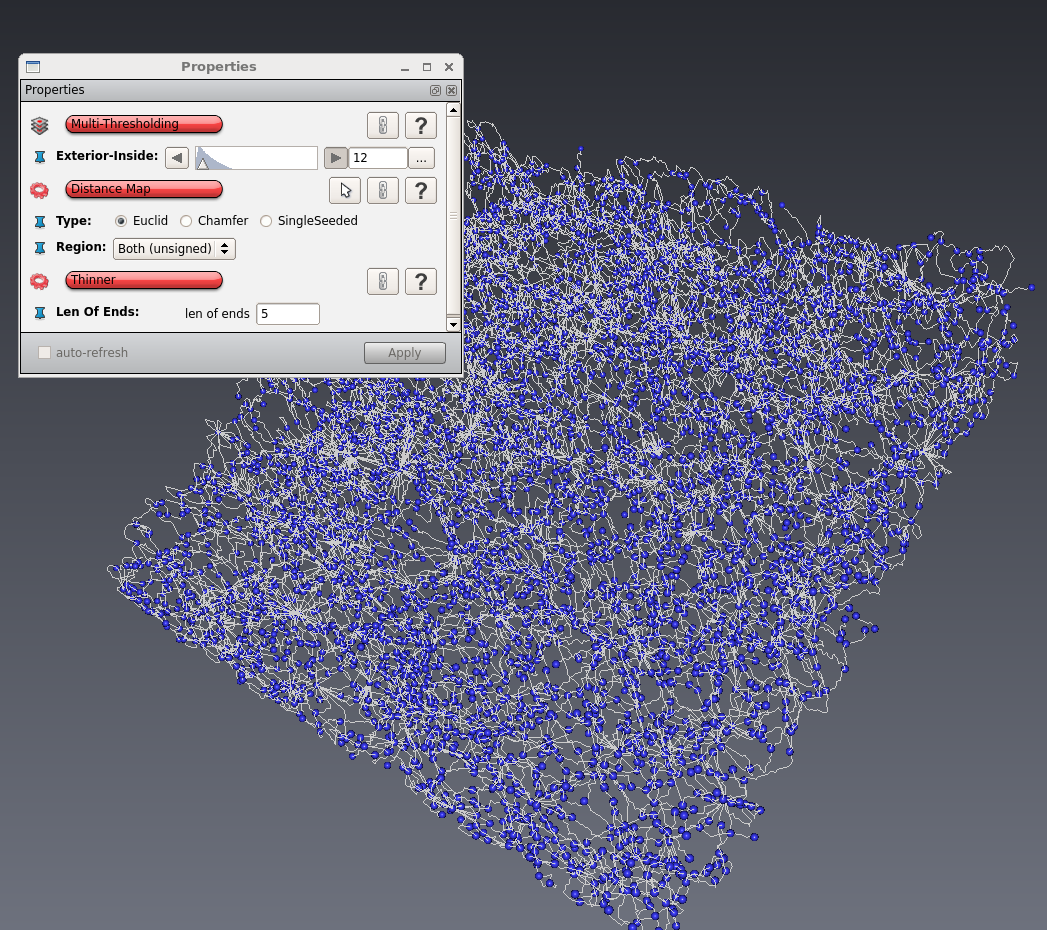
\includegraphics[width=1.0\textwidth]{Figures/chapter-image/avizo/ActinAllan11jun132_BIN12LEN5.png}%
        \end{center}

       \textsc{Network /}\\
       \textsc{Spatial Graph}
        };

      \node[blockimage] (C) at (1.5,0) {
      \textsc{Reconstruction}\\
      \textsc{Algorithm}
      };
      \node[blocknetwork] (F) at (0,3.5) {
      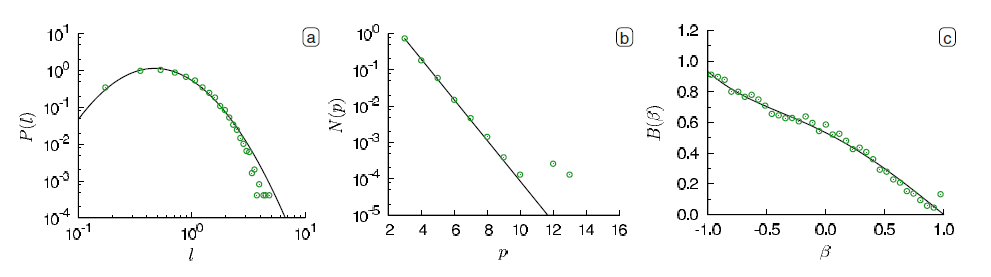
\includegraphics[width=1.0\textwidth]{Figures/chapter-reconstruct/lindstrom-paper-images.png}%

      \textsc{Statistics}
      };

      \node[blockmodel] (D) at (15,3) {\textsc{Modeling}};

      \draw[green,arrows={-triangle 45}] (A) -- (B);
      \draw[blue,arrows={-triangle 45}] (B) -- (F);
      \draw[blue,arrows={-triangle 45}] (F) -- (C);
      \draw[red,arrows={-triangle 45}] (B) -- (D);
      \draw[green,arrows={-triangle 45}] (C) -- (B);

    \end{tikzpicture}
  \end{center}
  \caption[Scheme of the thesis]{Scheme of the project. }
\end{figure}

\section{Future work}%
\label{sec:future_work}

\subsection{Network Formation}%
\label{sub:network_formation}

A simulation of network formation might be pursued in the future
  using a growing spatial graph, a dynamic population of cross-linker and monomers, and a persistence length parameter representing the stiffness of the biopolymer.

  The simulation will begin with a fixed set randomly distributed `embryonic' fibers, composed by two end-nodes and an edge between them. At each step of the simulation, a node which represents one end-point of a fiber, will be selected at random from the population, and will grow with a probability given by the current monomer population. If the grow occurs, the monomer population will be reduced --until depletion. The direction of the grow will depend on the comparison between the persistence length parameter and the position of edge points attached to that node. In this way stiff biopolymer will tend to grow in straight lines, and flexible chains will tend to bend.
  When two chains are close, and grows occurs, they will attach with a probability depending on the current population of cross-linkers. If the cross-link does not happen, the chain will grow without colliding. Also, at every step, every occupied position, by an edge point or a node, which is close to another occupied position will have a probability to attach depending again on the cross-link population. The network generation will stop when there are no monomer left. Optionally, another parameter will be a detachment probability of cross-linked fibers. Also pseudo-forces can be simulated where edges stores tension every time they attach to another fiber, and release that tension to their adjacent edges when they are released. This might shed some light into slow-dynamical processes and the quake-events behaviours reported TODO  This tension can also be added randomly to existing attached edges to simulate energy transfer from brownian movements of its components. After stability of the network we could study its graph properties, and compare them to the statistical distributions found in our image-extracted networks.

\subsection{Long time behaviour: network quakes and aging}
\label{sub:quakes}
There are reports in the literature \citep{kajiya_slow_2013}, and also by group
mates\citep{vincent_micro-rheological_2013}, that at long times, physical
biopolymer networks can be affected by sudden de-correlations that occur over a
few tenths of a second. The more plausible conjecture is that such quakes are associated with the release of
chain constraint due to unbinding of cross-links.  This is reported
experimentally in our group  with micro-rheology DWS techniques.
Current models of networks, such as the Glassy WLC model
\citep{kroy_glassy_2007}, cannot predict this behaviour \citep{vincent_micro-rheological_2013}.  A
computer simulation as sketched in \autoref{sub:network_formation} may shed some light on the topic.

It is also interesting the aging phenomena: the slow change of the physical
properties over time. This behaviour is related with non-ergodic systems and
with glassy systems, where long orders correlations(solids) no longer exists,
but there is still some local order.\citep{cipelletti_slow_????}

\subsection{ITKBoostGraph}%
\label{sub:itkboostgraph}

  The work done here about mapping between images and a spatial graph might be ported in the future to the image analysis library ITK as an external module to facilitate its adoption.

\subsection{Complex Networks Tools}%
\label{sub:complex_networks_tools}

The spatial graphs can be further analyzed with tools from the complex networks field, computing quantities like clustering and centrality are two lines of code away from the current status using the boost graph library (BGL). The graph can also be exported to the graphviz format (already implemented) to be used by any other network library if preferred.

\subsection{Public Database}%
\label{sub:public_database}

  I would like to set-up or contribute to a centralized public database of volumetric images of biopolymer networks. Optionally skeletonized images, and extracted spatial graphs would be associated.

